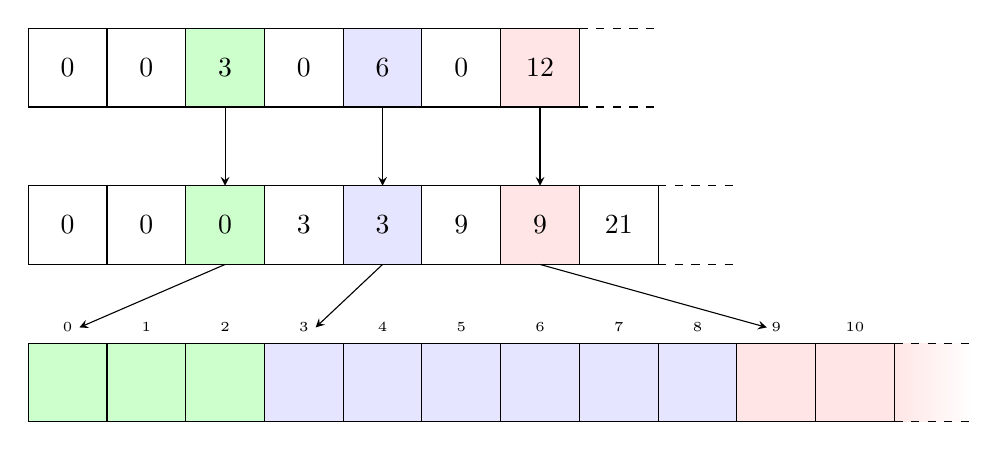
\begin{tikzpicture}[>=stealth]
\usetikzlibrary{fadings}

\draw[fill=green!20] (2,0) rectangle ++(1,1);
\draw[fill=blue!10] (4,0) rectangle ++(1,1);
\draw[fill=red!10] (6,0) rectangle ++(1,1);


\foreach \x/\val in {0/0,1/0,2/3,3/0,4/6,5/0,6/12}
{
  \draw (\x,0) rectangle ++(1,1);
  \draw node at (\x+0.5, 0.5) {\val};
}
\draw[dashed] (7,1) -- ++(1,0);
\draw[dashed] (7,0) -- ++(1,0);

\foreach \x in {2,4,6}
{
  \draw[->] (\x+0.5,0) -- ++(0,-1);
}

\draw[fill=green!20] (2,-2) rectangle ++(1,1);
\draw[fill=blue!10] (4,-2) rectangle ++(1,1);
\draw[fill=red!10] (6,-2) rectangle ++(1,1);

\foreach \x/\val in {0/0,1/0,2/0,3/3,4/3,5/9,6/9,7/21}
{
  \draw (\x,-2) rectangle ++(1,1);
  \draw node at (\x+0.5, -1.5) {\val};
}
\draw[dashed] (8,-1) -- ++(1,0);
\draw[dashed] (8,-2) -- ++(1,0);

\foreach \x in {0,...,2}
  \draw[fill=green!20] (\x,-4) rectangle ++(1,1);

\foreach \x in {3,...,8}
  \draw[fill=blue!10] (\x,-4) rectangle ++(1,1);

\foreach \x in {9,10}
  \draw[fill=red!10] (\x,-4) rectangle ++(1,1);

\fill [red!10,path fading=east] (11,-4) rectangle ++(1,1);

\draw[->] (2.5, -2) -- (0.65, -2.8);

\draw[->] (4.5, -2) -- (3.65, -2.8);
\draw[->] (6.5, -2) -- (9.38, -2.8);


\foreach \x in {0,...,10}
{
  \draw (\x,-4) rectangle ++(1,1);
  \draw[font=\tiny] node at (\x+0.5, -2.8) {\x};
}

\draw[dashed] (11,-3) -- ++(1,0);
\draw[dashed] (11,-4) -- ++(1,0);


\end{tikzpicture}